\documentclass[10pt,aspectratio=43,mathserif]{beamer}		
%设置为 Beamer 文档类型,设置字体为 10pt,长宽比为16:9,数学字体为 serif 风格

%%%%-----导入宏包-----%%%%
\usepackage{ccnu}			%导入 CCNU 模板宏包
%\usepackage{ctex}			 %导入 ctex 宏包,添加中文支持
\usepackage{xeCJK}
\usepackage{amsmath,amsfonts,amssymb,bm}   %导入数学公式所需宏包
\usepackage{color}			 %字体颜色支持
\usepackage{graphicx,hyperref,url}	
%%%%%%%%%%%%%%%%%%


% \setsansfont{Helvetica} 							%Windows和Mac OS下都可用
\setsansfont{Times New Roman}
\setCJKmainfont{Microsoft YaHei}   	%仅Windows可用
% \setCJKmainfont{Songti SC}								%仅Mac OS下可用

\beamertemplateballitem		%设置 Beamer 主题


\AtBeginSection[]
{
  \begin{frame}<beamer>
    \frametitle{\textbf{目录}}
    \textbf{\tableofcontents[currentsection]}
  \end{frame}
}


%%%%----首页信息设置----%%%%
% \title[Sending out an SMS]{\fontsize{13pt}{18pt}\selectfont {Sending out an SMS: Characterizing the Security of the SMS Ecosystem with Public Gateways}}
% \subtitle{\fontsize{9pt}{14pt}\selectfont \textbf{利用公共网关的SMS生态系统的安全性描述}}	

\title[基于NSCT-SF-PCNN图像融合算法实现]{\fontsize{13pt}{18pt}\selectfont \textbf{基于NSCT-SF-PCNN图像融合算法实现}}	
%%%%----标题设置


\author[H. Wang]{
  王欢
  \\
  {\small {学号:181499}} \\
  {\small {指导教师:金立左}}}
%%%%----个人信息设置

\institute[SEUAuto]{
  东南大学自动化学院}
%%%%----机构信息

\date[\today]{
 \today}
%%%%----日期信息


\begin{document}

\begin{frame}
\titlepage
\end{frame}				%生成标题页



\section*{目录}

		\begin{frame}
		\frametitle{\textbf{目录}}
		\textbf{\tableofcontents}
		\end{frame}				%生成提纲页

\section{引言}
%%%%%%%%%%%%%%%%%%%%%%%%%%%%%%%%%%%%%%%%%%%%%%%%%%%%%%%%%%%%%%%%%%%%%%%%%%%%%%%%%%%%%%%%%%%%%%%%%%%%%%%%%%%%%%%%%%
		\begin{frame}
			\frametitle{\textbf{引言}}
            \begin{block}{\textbf{研究背景}}
                \begin{itemize}
                    \item 多传感器图像融合
                    \item 多焦点图像融合
                    \item 时间序列图像融合
                \end{itemize}
            \end{block}

            \begin{block}{\textbf{主要工作}}
                \begin{itemize}
                    \item 多源图像配准
                    \item 图像特征分解
                    \item 图像重构
                \end{itemize}
            \end{block}
        \end{frame}

\section[NSCT]{NSCT的图像融合方法}
%%%%%%%%%%%%%%%%%%%%%%%%%%%%%%%%%%%%%%%%%%%%%%%%%%%%%%%%%%%%%%%%%%%%%%%%%%%%%%%%%%%%%%%%%%%%%%%%%%%%%%%%%%%%%%%%%%%
    \begin{frame}
		  \frametitle{\textbf{图像融合中的Contourlet理论}}
            \begin{columns}
                \column{.5\textwidth}
                \footnotesize
                Contourlet变换是利用拉普拉斯金字塔(LP)变换和方向滤波器组(Directional Filter Bank, DFB)实现的一种图像多尺度几何分析工具,
它不仅具有多分辨率和时频局部性的特点,还具有高度的方向性和各向异性。Contourlet变换将多尺度分析和方向分析分开进行,分解为LP分解和DFB滤波两个过程,
重构则是上述两个过程的逆过程。

LP首先用于捕获点不连续性,然后是DFB,以将点不连续性链接到线性结构。相较于小波变换,Contourlet的灵活性体现在每层分解方向数量可以不同。
不幸的是,原始Contourlet变换的LP和DFB中都存在下采样操作(如右图所示),因此在进行平移变换时,容易产生\textbf{频谱混叠现象}。

                \column{.5\textwidth}
                \begin{figure}[!t]
                    \centering
                    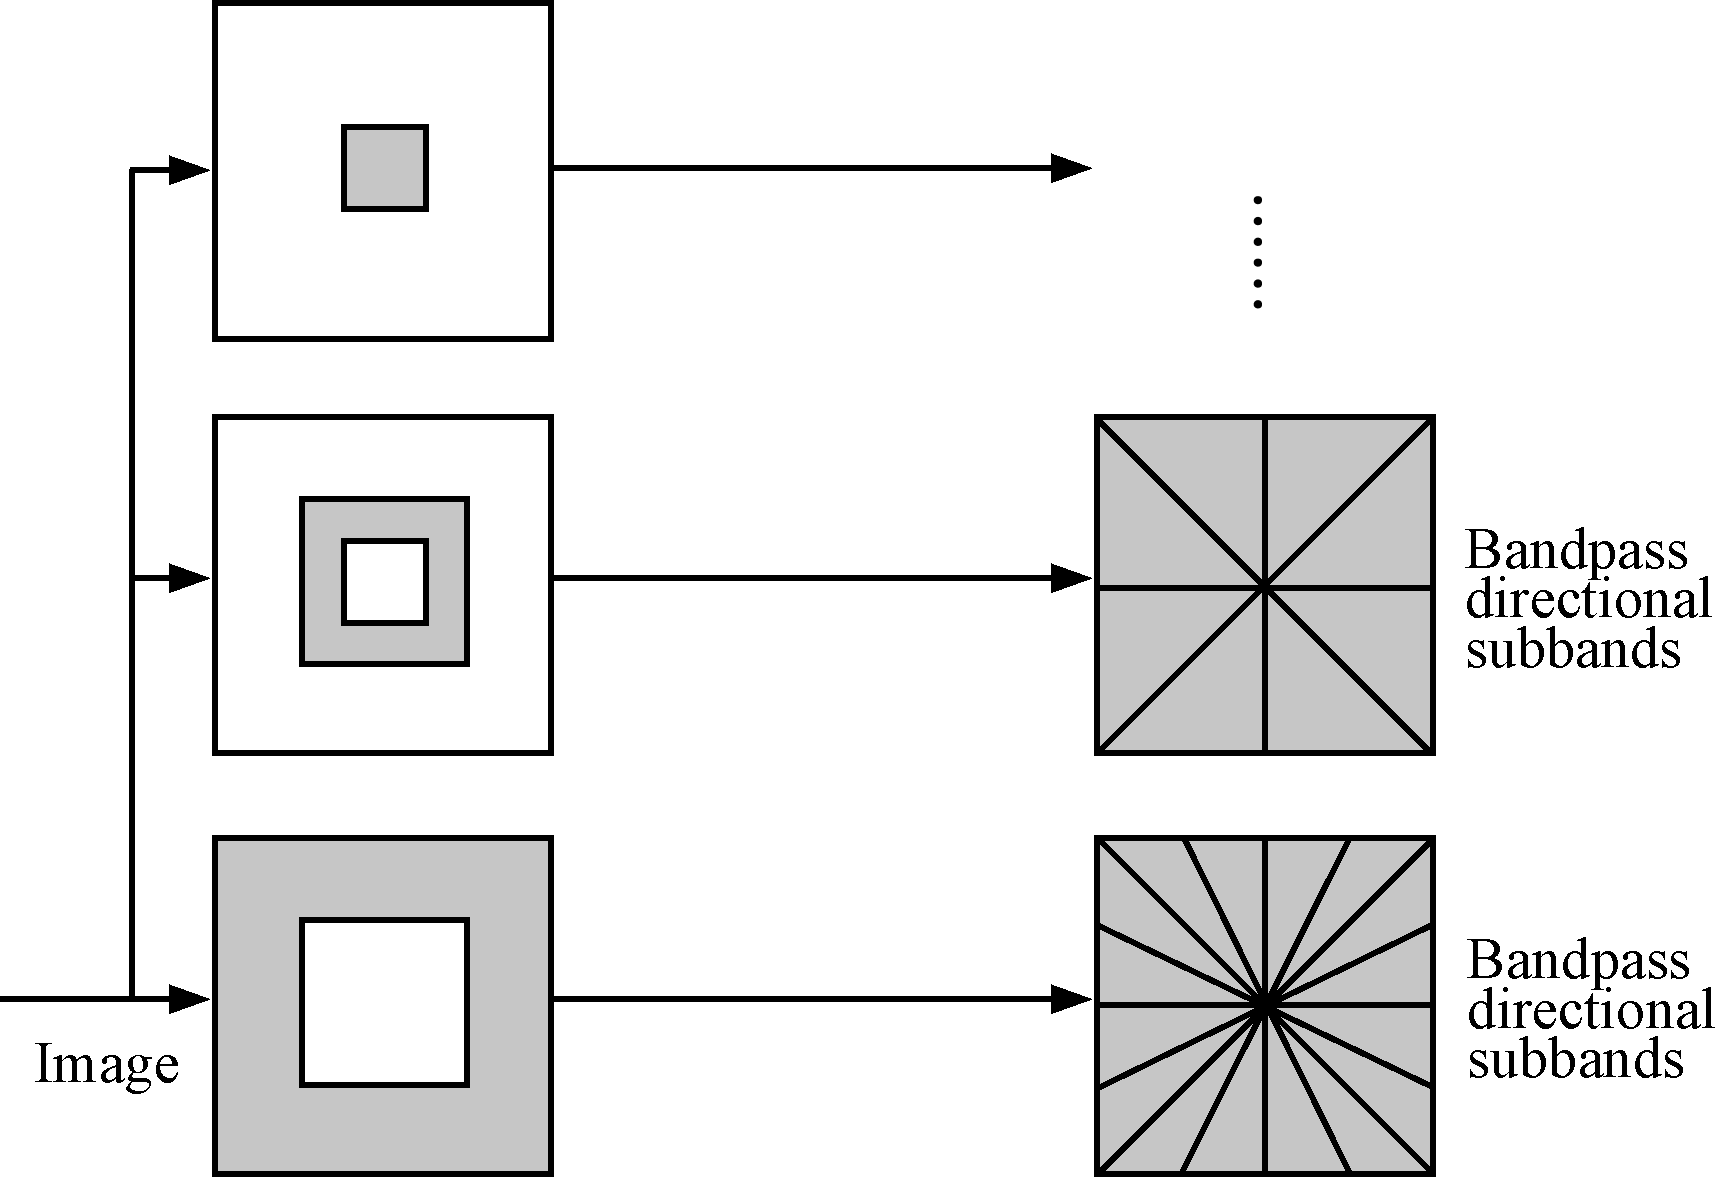
\includegraphics[width=1.1\textwidth]{./figures/nsct/Contourlet.png}
                    \caption{Contourlet}
                    \label{fig:CTandNSCT}
                \end{figure}
        \end{columns}
    \end{frame}
%%%%%%%%%%%%%%%%%%%%%%%%%%%%%%%%%%%%%%%%%%%%%%%%%%%%%%%%%%%%%%%%%%%%%%%%%%%%%%%%%%%%%%%%%%%%%%%%%%%%%%%%%%%%%%
    \begin{frame}
		  \frametitle{\textbf{NSCT}}
            \begin{columns}
                \column{.5\textwidth}
                \footnotesize
                为克服Contourlet的频谱混叠缺点,Cunha 等人提出的非下采样 Contourlet 变换
(NSCT)属于完全冗余 Contourlet 变换(如右图所示),即塔式变换和方向变换均冗余,它利用非下
采 样 金 字 塔(Nonsubsampled Pyramid , NSP ) 变换和非下采样方向滤波器组
(Nonsubsampled Directional Filter Bank,NSDFB)构造,具有完全平移不变性,且图像
经 NSCT 分解后得到的各子带系数的尺寸大小与源图像是相同的,这有利于图像融合时
融合规则的制定。与 Contourlet 变换类似,NSCT 同样将多尺度分析和方向分析分开进行。

                \column{.5\textwidth}
                \begin{figure}[!t]
                    \centering
                    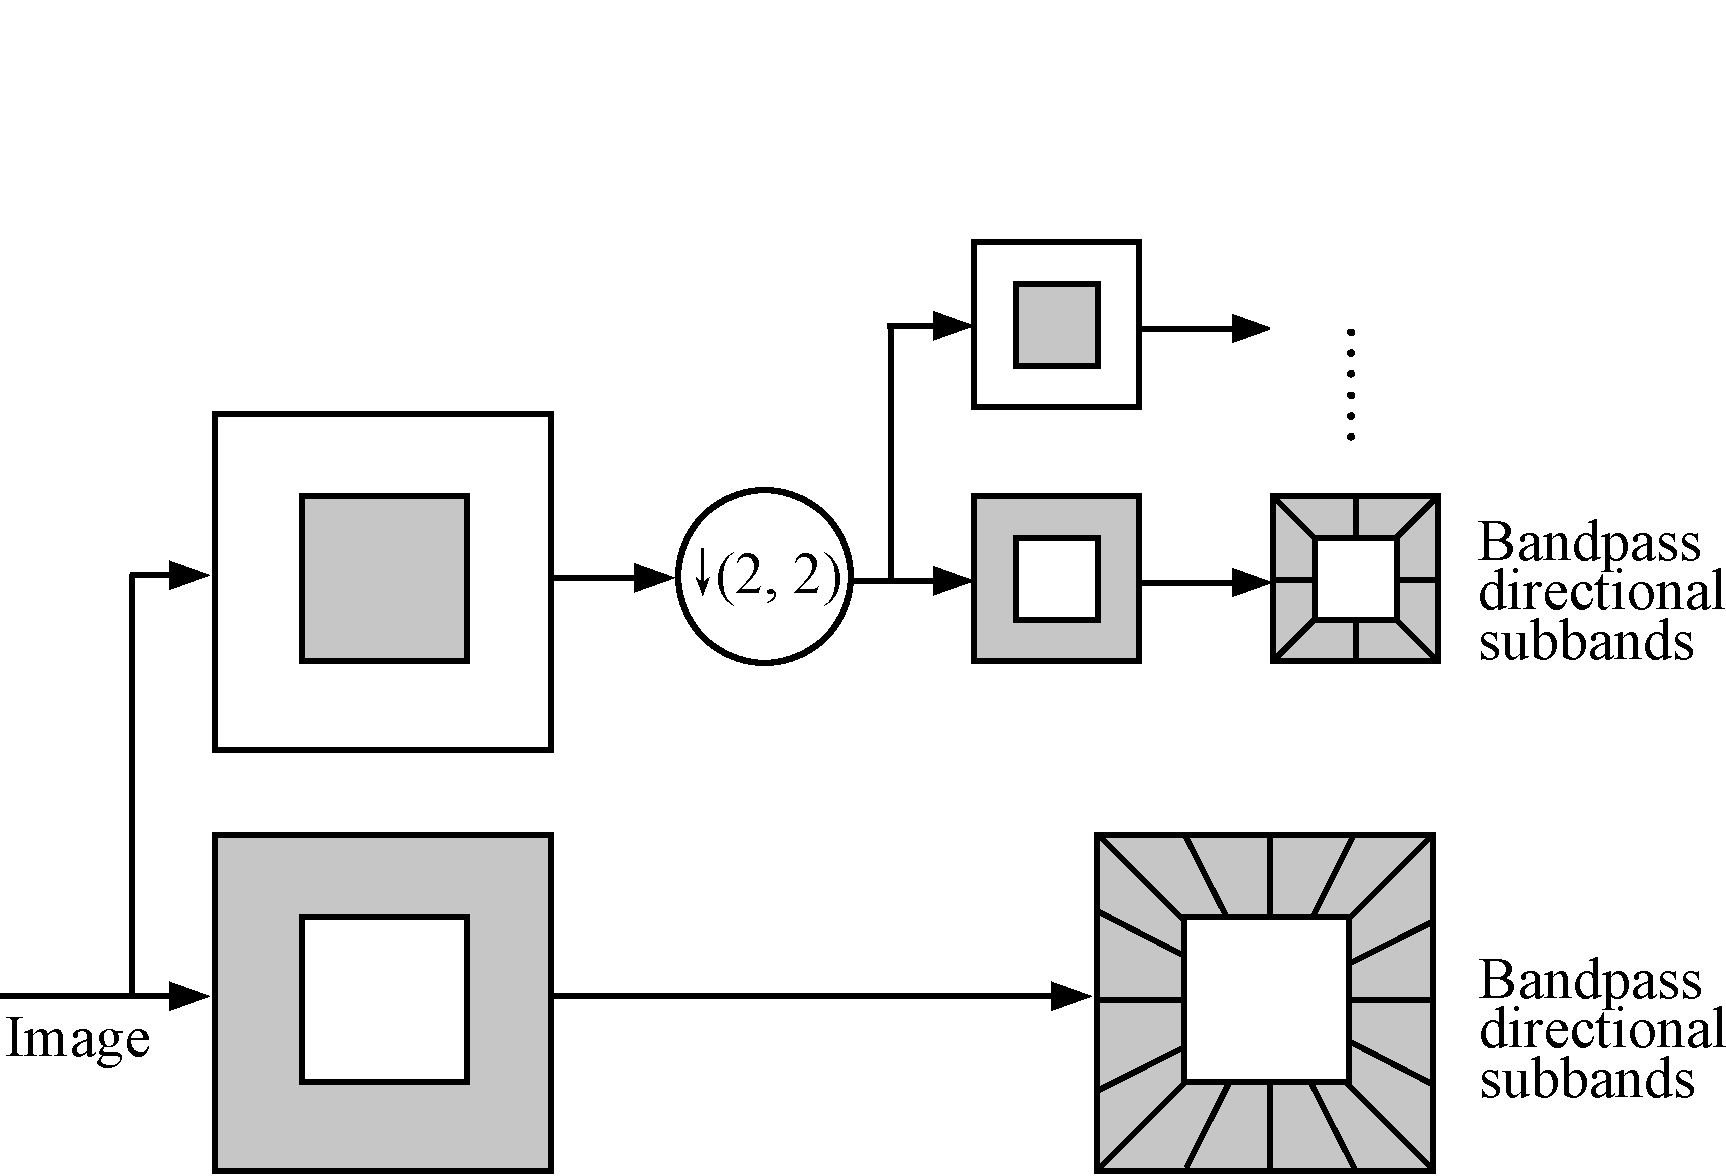
\includegraphics[width=1.1\textwidth]{./figures/nsct/NSCT-struct.png}
                    \caption{Contourlet}
                    \label{fig:CTandNSCT}
                \end{figure}
        \end{columns}
    \end{frame}
%%%%%%%%%%%%%%%%%%%%%%%%%%%%%%%%%%%%%%%%%%%%%%%%%%%%%%%%%%%%%%%%%%%%%%%%%%%%%%%%%%%%%%%%%%%%%%%%%%%%%%
    \begin{frame}
		  \frametitle{\textbf{非下采样金字塔(NSP)变换}}
            \begin{columns}
                \column{.5\textwidth}
                \footnotesize
                NSP 采用的是一组二维的双通道非下采样滤波器组(Nonsubsampled Filter Bank,
NSFB),实现一个类似于 Contourlet 变换中 LP 变换的子带分解。使用 NSP 对图像进行
分解时,在每一级 NSP 分解后,都需要用矩阵 $2I$ 对滤波器进行填零上采样,作为下一
级分解的滤波器,其中 $I$ 为 2 阶单位矩阵。右图展示了图像经 3 级 NSP 分解的过程,
其中$y_0$为低频子带,$y_1$、$y_2$、$y_3$为高频子带,浅灰色区域为上采样造成的混叠,从图中可以看出各子带图像具有相同的尺寸大小。

                \column{.5\textwidth}
                \begin{figure}[!t]
                    \centering
                    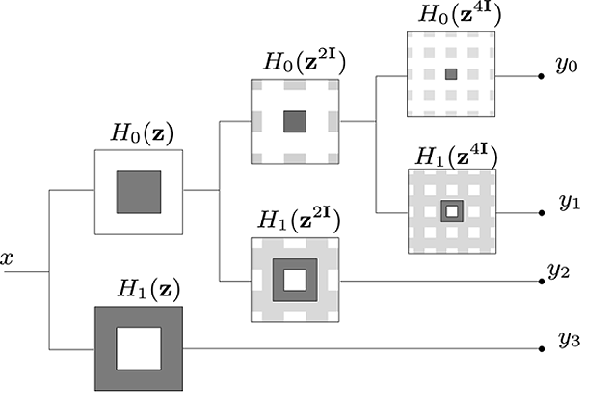
\includegraphics[width=1.1\textwidth]{./figures/nsct/NSP.png}
                    \caption{NSP分解示意图}
                \end{figure}
        \end{columns}
    \end{frame}
%%%%%%%%%%%%%%%%%%%%%%%%%%%%%%%%%%%%%%%%%%%%%%%%%%%%%%%%%%%%%%%%%%%%%%%%%%%%%%%%%%%%%%%%%%%%%%%%%%%%%%%%%%%%%%%%%%%
\begin{frame}
		  \frametitle{\textbf{非下采样方向滤波器组(NSDFB)}}
            \begin{columns}
                \column{.5\textwidth}
                \footnotesize
                NSDFB 采用的同样也是一组二维的双通道 NSFB。NSDFB 对图像进行树形结构分
解,在每一级方向分解后,都需要用一个梅花采样矩阵对 DFB 中的所有滤波器进行填
零上采样,作为下一级方向分解的 DFB。右图展示了一个四通道的 NSDFB 的结构,
它由两个双通道扇形 QFB 经过填零上采样操作得到。

                \column{.5\textwidth}
                \begin{figure}[!t]
                    \centering
                    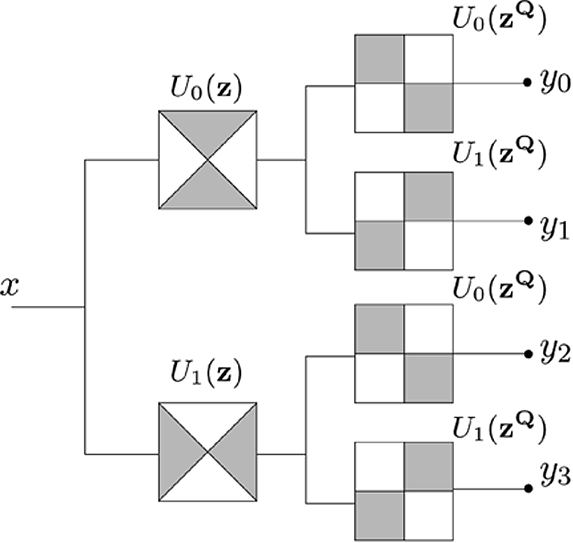
\includegraphics[width=1.1\textwidth]{./figures/nsct/NSDFB.png}
                    \caption{四通道NSDFB}
                \end{figure}
        \end{columns}
    \end{frame}
%%%%%%%%%%%%%%%%%%%%%%%%%%%%%%%%%%%%%%%%%%%%%%%%%%%%%%%%%%%%%%%%%%%%%%%%%%%%%%%%%%%%%%%%%%%%%%%%%%%%%%%%%%%%%%%
\begin{frame}
		  \frametitle{\textbf{由NSP和NSDFB构建NSCT}}
            \begin{columns}
                \column{.5\textwidth}
                \footnotesize
将 NSP 和 NSDFB 结合起来就可以构造 NSCT。

                \column{.5\textwidth}
                \begin{figure}[!t]
                    \centering
                    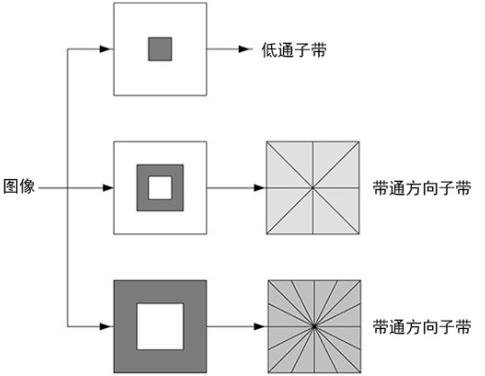
\includegraphics[width=1.1\textwidth]{./figures/nsct/NSCT-NSFB.png}
                    \caption{构建NSCT所采用的NSFB结构}
                \end{figure}
        \end{columns}
    \end{frame}

%%%%%%%%%%%%%%%%%%%%%%%%%%%%%%%%%%%%%%%%%%%%%%%%%%%%%%%%%%%%%%%%%%%%%%%%%%%%%%%%%%%%%%%%%%%%%%%%%%%%%%%%%%%
\begin{frame}
		  \frametitle{\textbf{NSCT中消除频谱混叠现象}}
            \begin{figure}[!t]
            \centering
            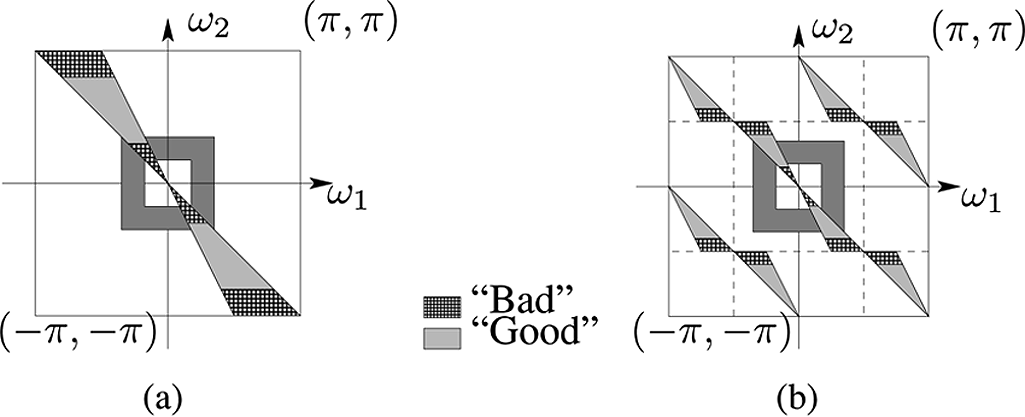
\includegraphics[width=4in]{./figures/nsct/NSCT_eliminate_aliasing.png}
            \end{figure}
            在构建 NSCT 时,
由于 NSDFB 树状结构的特性,对 NSP 分解得到的高频子带使用 NSDFB 时,在较低和
较高频率上的方向响应存在混叠,如图(a)所示,在方向滤波器的通带区域上标
注了“Good”或“Bad”,较粗尺度下的高通通道将被方向滤波器中的“Bad”通带区
域过滤掉,这使得丢失大量的方向信息,导致图像严重走样。如果适当地对 NSDFB 上
采样处理,就能将“Good”通带区域覆盖到高通通道上,如图(b)所示。
		\end{frame}
%%%%%%%%%%%%%%%%%%%%%%%%%%%%%%%%%%%%%%%%%%%%%%%%%%%%%%%%%%%%%%%%%%%%%%%%%%%%%%%%%%%%%%%%%%%%%%%%%%%%%
\begin{frame}
		  \frametitle{\textbf{NSP和NSDFB完全重构的条件}}
            \begin{figure}[ht] %figure参数:h 此处(here)t 页顶(top)b 页底(bottom)p 独立一页(page)
	\begin{minipage}[t]{0.5\linewidth}%需要几张添加即可,注意设定合适的linewidth
		\centering
		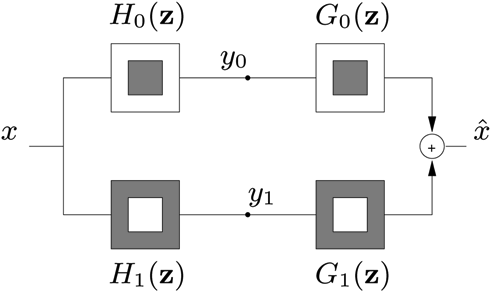
\includegraphics[width=0.8\linewidth]{./figures/nsct/NSFB_struct(a).png}
		\setlength{\abovecaptionskip}{5pt}
		\setlength{\belowcaptionskip}{5pt}
		\caption{塔形NSFB}
		\label{fig:NSFB_struct(a)}
	\end{minipage}%
	\begin{minipage}[t]{0.5\linewidth}
		\centering
		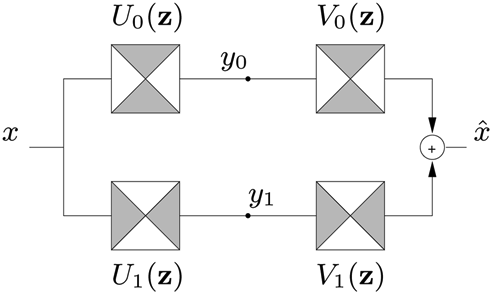
\includegraphics[width=0.8\linewidth]{./figures/nsct/NSFB_struct(b).png}
		\setlength{\abovecaptionskip}{5pt}
		\setlength{\belowcaptionskip}{5pt}
		\caption{扇形NSFB}
		\label{fig:NSFB_struct(b)}
	\end{minipage}
\end{figure}
并且必
须满足如下式所示的 Bezout 恒等式,才能保证 NSP 和 NSDFB 是完全重构的,继而
保证 NSCT 是完全重构的。
            \begin{equation*}
                \begin{aligned}
                H_0(z)G_0(z)+H_1(z)G_1(z) &= 1\\
                U_0(z)V_0(z)+U_1(z)V_1(z) &= 1
                \end{aligned}
            \end{equation*}
		\end{frame}
%%%%%%%%%%%%%%%%%%%%%%%%%%%%%%%%%%%%%%%%%%%%%%%%%%%%%%%%%%%%%%%%%%%%
\begin{frame}
		  \frametitle{\textbf{NSCT分解结果}}
            \begin{columns}
                \column{.5\textwidth}
                \footnotesize
以 Zoneplate 作为输入图像(如右图所示),经两层 NSP
变换分解,尺度从细到粗的方向分解级数分别为 1、2。

                \column{.5\textwidth}
                \begin{figure}[!t]
                    \centering
                    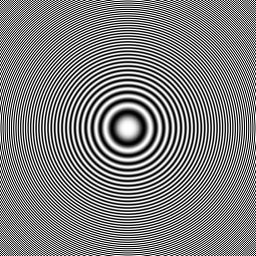
\includegraphics[width=0.8\textwidth]{./figures/nsct/Zoneplate.png}
                    \caption{Zoneplate原始图像}
                \end{figure}
        \end{columns}
    \end{frame}
%%%%%%%%%%%%%%%%%%%%%%%%%%%%%%%%%%%%%%%%%%%%%%%%%%%%%%%%%%%%%%%%%%%%%%%%%%%%%%%%%%%%%%%%%%%%%
		\begin{frame}
		  \frametitle{\textbf{NSCT分解结果}}
            \begin{figure}[ht] %figure参数:h 此处(here)t 页顶(top)b 页底(bottom)p 独立一页(page)
	\centering
	\begin{minipage}[t]{0.4\linewidth}%需要几张添加即可,注意设定合适的linewidth
		\centering
		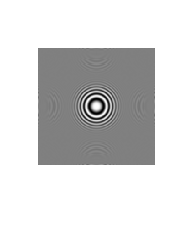
\includegraphics[width=0.6\linewidth]{./figures/nsct/NSCT_de_a.png}

		\caption{低频子带}
		\label{fig:NSCT_de_a}
	\end{minipage}%
	\begin{minipage}[t]{0.4\linewidth}
		\centering
		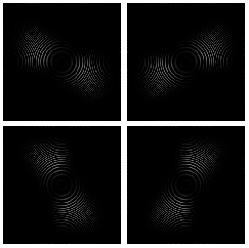
\includegraphics[width=0.6\linewidth]{./figures/nsct/NSCT_de_b.png}

		\caption{第1层高频方向子带}
		\label{fig:NSCT_de_b}
	\end{minipage}
	\\
	\begin{minipage}[t]{0.7\linewidth}
		\centering
		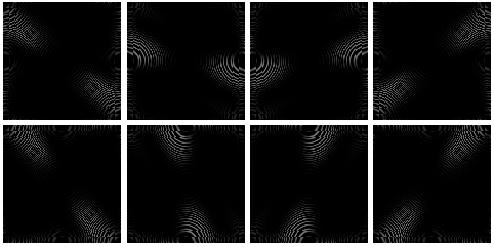
\includegraphics[width=0.7\linewidth]{./figures/nsct/NSCT_de_c.png}

		\caption{第2层高频方向子带}
	\end{minipage}
\end{figure}
		\end{frame}
%%%%%%%%%%%%%%%%%%%%%%%%%%%%%%%%%%%%%%%%%%%%%%%%%%%%%%%%%%%%%%%%%%%%%%%%%%%%%%%%%%%%%%%%%%%%%%%%%%%%%%%%%%%
%%%%%%%%%%%%%%%%%%%%%%%%%%%%%%%%%%%%%%%%%%%%%%%%%%%%%%%%%%%%%%%%%%%%%%%%%%%%%%%%%%%%%%%%%%%%%%%%%%%%%%%%%%%%
\section[PCNN]{基于脉冲耦合神经网络的图像融合算法}

		\begin{frame}
		  \frametitle{\textbf{PCNN简化模型}}
          由于原始PCNN模型较为复杂,且模型参数物理意义并不明确,因此实际使用时模型经过简化。
其中,$\bigotimes$为卷积运算,$\bigoplus$为加法运算,$i$、$j$为神经元标号,其连接范围为$k$、$l$,
$S$为神经元外部激励,本文中即图像灰度值,直接作为神经元的反馈输入$F$,
$L$为神经元连接输入,其连接矩阵、放大系数和衰减时间系数分别为$W$、$V_L$和$\alpha _L$,
$U$为神经元内部活动项,其连接强度系数为$\beta$,
$\theta$为动态门限, 其放大系数和衰减时间系数分别为$V_{\theta}$和$\alpha _{\theta}$,
$Y$为神经元输出,当$U>\theta$时产生一次输出。
            \begin{equation*}
            \begin{aligned}
            F_{ij}(n) &= S_{ij}
            \\
            L_{ij}(n) &= e^{-\alpha _L} L_{ij}(n-1) + V_L \sum_{kl} W_{ij,kl}Y_{kl}(n-1)
            \\
            U_{ij}(n) &= F_{ij}(n) (1+\beta L_{ij}(n))
            \\
            \Theta _{ij}(n) &=e^{-\alpha _\theta} \Theta _{ij}(n-1) + V_\theta Y_{ij}(n-1)
            \\
            Y_{ij}(n) &= \left\{\begin{matrix}1, ~ U_{ij}(n) \geq \Theta _{ij}(n)\\ 0, ~ U_{ij}(n) < \Theta _{ij}(n)\end{matrix}\right.
            \end{aligned}
            \end{equation*}
		\end{frame}
%%%%%%%%%%%%%%%%%%%%%%%%%%%%%%%%%%%%%%%%%%%%%%%%%%%%%%%%%%%%%%%%%%%%%%%%%%%%%%%%%%%%%%%%%%%%%%%%%%%%%%%%%%%%%%%%
\begin{frame}
		  \frametitle{\textbf{PCNN简化示意图}}
            \begin{columns}
                \column{.5\textwidth}
                \begin{figure}[!t]
                    \centering
                    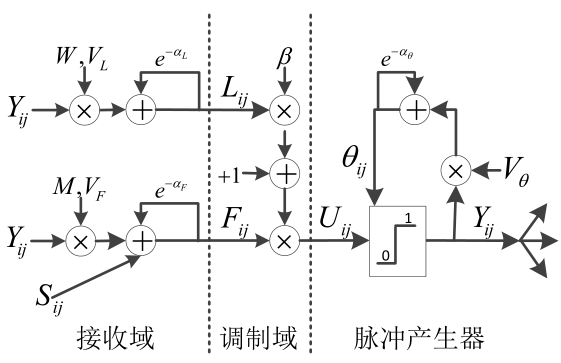
\includegraphics[width=0.8\textwidth]{./figures/pcnn/PCNN-sample.png}
                    \caption{PCNN神经元简化模型}
                \end{figure}

                \column{.5\textwidth}
                \begin{figure}[!t]
                    \centering
                    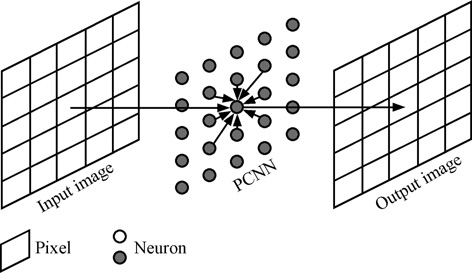
\includegraphics[width=0.8\textwidth]{./figures/pcnn/PCNN-image-proc.png}
                    \caption{PCNN图像处理示意图}
                \end{figure}
        \end{columns}
    \end{frame}

%%%%%%%%%%%%%%%%%%%%%%%%%%%%%%%%%%%%%%%%%%%%%%%%%%%%%%%%%%%%%%%%%%%%%%%%%%%%%%%%%%%%%%%%%%%%%%%%%%%%%%%%
\begin{frame}
		  \frametitle{\textbf{PCNN工作原理}}
        PCNN图像融合流程如图所示。根据PCNN工作原理可知,经过一定次数迭代过后可得双源图像点火映射图,通过判决选择算子计算融合图像系数,进而融合图像。
        \begin{figure}[!t]
            \centering
            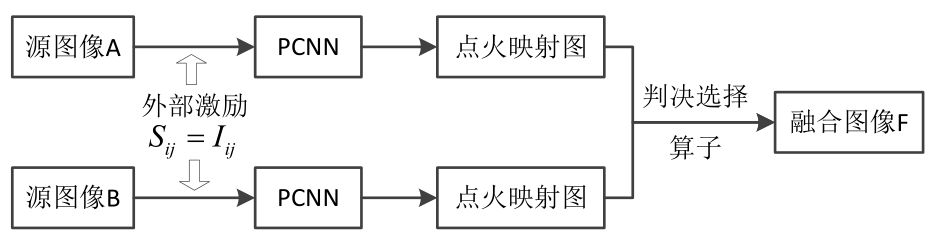
\includegraphics[width=4in]{./figures/pcnn/PCNN-fusion.png}
            \end{figure}
    \end{frame}


\begin{frame}
		  \frametitle{\textbf{算子选择}}
        当PCNN模型确定后,只需确定判决选择算子,设双源图像$A$和$B$的$n$次点火映射图分别为$T_{ij}^A(n)$和$T_{ij}^B(n)$,融合图像为$F$,$I_{ij}$为图像$(i,j)$处像素灰度值,则有:
        \begin{equation*}
I_{ij}^F = \left\{\begin{matrix}
I_{ij}^A ,~ T_{ij}^A(n) \geq T_{ij}^B(n)\\ 
I_{ij}^B ,~ T_{ij}^A(n) < T_{ij}^B(n)
\end{matrix}\right.
\end{equation*}
\end{frame}
%%%%%%%%%%%%%%%%%%%%%%%%%%%%%%%%%%%%%%%%%%%%%%%%%%%%%%%%%%%%%%%%%%%%%%%%%%%%%%%%%%%%%%%%%%%%%%%%%%%%%%%%%%%%%%%
%%%%%%%%%%%%%%%%%%%%%%%%%%%%%%%%%%%%%%%%%%%%%%%%%%%%%%%%%%%%%%%%%%%%%%%%%%%%%%%%%%%%%%%%%%%%%%%%%%%%%%%%%%%%%%%
\section[NSCT-SF-PCNN]{基于NSCT-SF-PCNN的图像融合算法}
    
        \begin{frame}
		  \frametitle{\textbf{NSCT-SF-PCNN算法框架}}
			PCNN用于图像融合的核心原因在于其神经元的全局耦合和脉冲同步。 
这些生物特征充分利用了图像中的局部信息,而不是大多数流行的基于MSD的融合算法中的单一系数信息。 
尽管在多焦点图像融合中研究了PCNN的区域点火特性,但仍然使用点火时间作为选择NSCT系数的确定。

\begin{figure}[ht] %figure参数:h 此处(here)t 页顶(top)b 页底(bottom)p 独立一页(page)
	\centering
	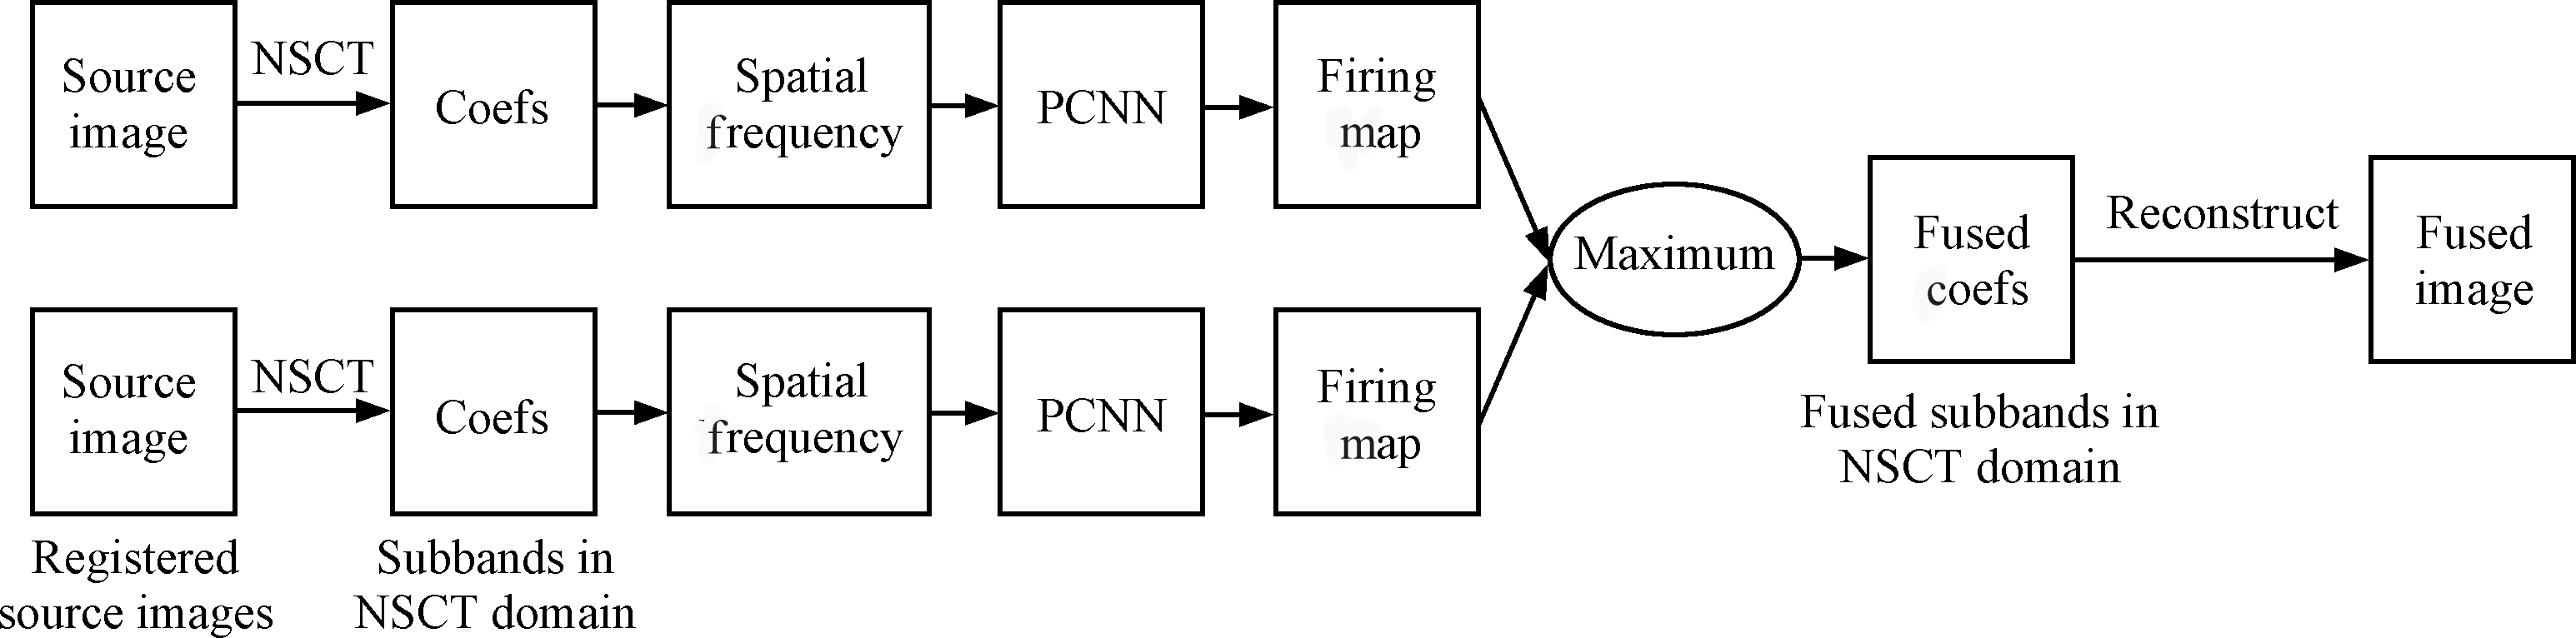
\includegraphics[width=0.8\linewidth]{./figures/pcnn/NSCT-SF-PCNN.png} %片文件的相对路径
\end{figure}
		\end{frame}

        \begin{frame}
		  \frametitle{\textbf{NSCT-SF-PCNN算法实现}}
			\begin{enumerate}
  \item Decompose the source images into subbands via NSCT.
  \item Measure the SF as (1) in slipping window of coefficients in subbands.
  \item SF in each subbands are input to PCNN to motivate the neurons and generate pulse of neurons with (2). Then, firing times $T_{ij}^{l,k}(n)$ is calculated as (3).
  \item Get the decision map $D_{ij}^{l,k}$based on (4) and select the coefficients with (5), which means that coefficients with large firing times are selected as coefficients of the fused image.
    \begin{equation}
        D_{F,ij}^{l,k}=\left\{
        \begin{array}{rcl}
        1 & & {T_{1,ij}^{l,k}(n) \geq T_{2,ij}^{l,k}(n)}\\
        0 & & {T_{1,ij}^{l,k}(n) < T_{2,ij}^{l,k}(n)}
        \end{array} \right.
    \end{equation}
    \begin{equation}
        x_{F,ij}^{l,k}=\left\{
        \begin{array}{rcl}
        x_{1,ij}^{l,k} & & {D_{ij}^{l,k}(n)=1}\\
        x_{2,ij}^{l,k} & & {D_{ij}^{l,k}(n)=0}
        \end{array} \right.
    \end{equation}
    where $x_{F,ij}^{l,k}$,$x_{1,ij}^{l,k}$ and $x_{2,ij}^{l,k}$ denote the coefficients of the fused image and two source images, respectively.
  \item Use the selected-out coefficients in (5) to reconstruct the fused image via inverse NSCT.
\end{enumerate}
		\end{frame}

\begin{frame}
		  \frametitle{\textbf{NSCT-SF-PCNN算法Matlab实现}}
NSCT的具体参数为$\left[0,1,3,4,4\right]$。PCNN具体参数为:$\alpha_{L}=0.06931$,$\alpha_{\theta}=0.2$,$\beta=0.2$,$V_L=1.0$,$V_{\theta}=20$,
$W=\left[\begin{matrix}
   0.707 & 1 & 0.707 \\
   1 & 0 & 1 \\
   0.707 & 1 & 0.707
\end{matrix}\right]
$,最大迭代数为$n=200$.
		\end{frame}


\begin{frame}
		  \frametitle{\textbf{NSCT-SF-PCNN算法融合效果}}
\begin{figure}[ht] %figure参数:h 此处(here)t 页顶(top)b 页底(bottom)p 独立一页(page)
	\centering
	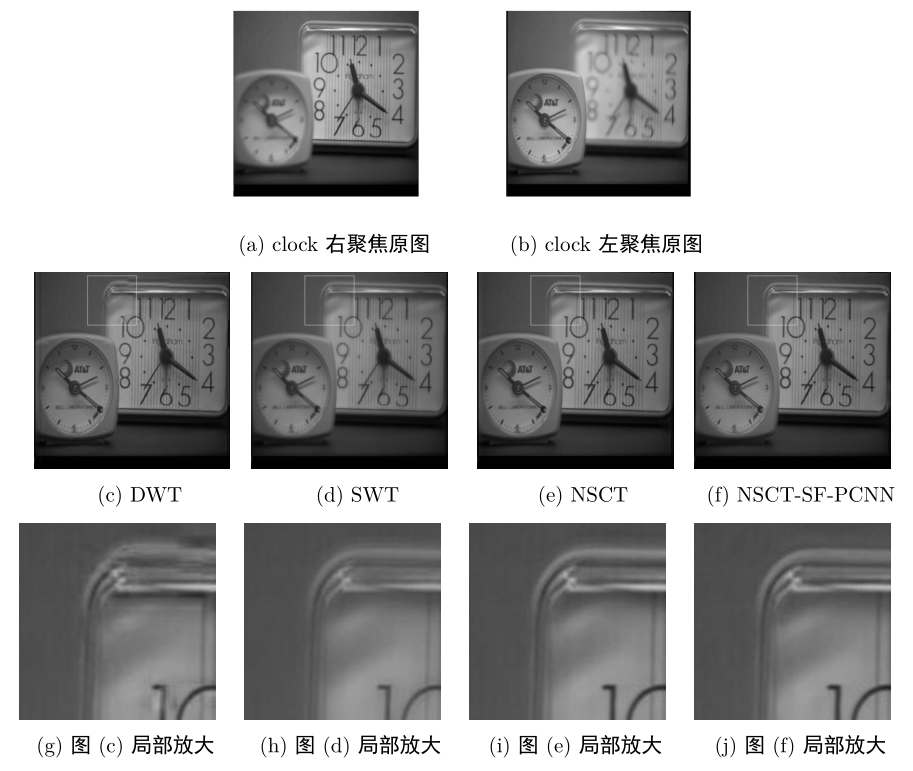
\includegraphics[width=0.8\linewidth]{./figures/pcnn/total.png} %片文件的相对路径
\end{figure}
		\end{frame}

\begin{frame}
		  \frametitle{\textbf{结果分析}}

\begin{enumerate}
\item 基于NSCT-SF-PCNN的图像融合算法有效地保留了左聚焦图像和右聚焦图像中的
目标信息
\item SWT 和 NSCT 分解时都没有下采样环节,使得变换都具有平移不变性,从而避免了伪 Gibbs 现象的出现
\item NSCT在方向分解上比 SWT 能获得更多的高频方向子带,捕获图像边缘的能力更强
\item 使用 NSCT 与 PCNN结合的图像融合方法,不但能捕获更多的边缘信息,而且能增强图像的对比度,使图像的边缘更加尖锐轮廓更加清晰,其中使用本文方法的融合图像最为明显
\end{enumerate}
\begin{block}{\textbf{总结}}
                基于NSCT-SF-PCNN的融合方法,不但能有效地融合多聚焦图像中的目标信息,还能增强图像的对
比度,更好地区分图像中的目标信息和背景信息。
            \end{block}
		\end{frame}



\section*{}
            \begin{frame}

                \begin{center}
                    \begin{minipage}{1\textwidth}
                        \setbeamercolor{mybox}{fg=white, bg=black!60!green}
                        \begin{beamercolorbox}[wd=0.70\textwidth, rounded=true, shadow=true]{mybox}
                        \LARGE \centering Thanks for Listening.
                        \end{beamercolorbox}
                    \end{minipage}
                \end{center}
                

            \end{frame}

\end{document} 